\documentclass[../main.tex]{subfiles} % required, if the Chapter be a seperate doc

\begin{document}

\section{Statistik}\label{sec:statistik}

\begin{itemize}ß
    \item \textmathbar{x} - Arithmetischer Mittelwert
    \item $\Delta$h - länge der gespanten Feder vom start der Messung Ohne belastung
    \item s - Standartabweichung des Einzelwertes
    \item $\Delta$\textmathbar{x} - Standartabweichtung des Mittelwertes
    \item r - Relativer Fehler
    \item D - Federkonstante
    \item R\textsuperscript{2} - Korrelationskoeffizient
\end{itemize}

\subsection{Kraft berechnung}\label{subsec:force-calculation}

Die Kraft wurde mit der Newtonischen Formel berechnet

$$ F = m * a $$

$a$ ist in diesem fall die Gravitation der Erde: 9.81 m/s\textsuperscript{2}

\begin{center}
    \begin{tabular}{ |l|l| } \hline\rowcolor{Gray!50}
        Masse [g] & Kraft [N] \\\hline
        0.00      & 0.0000    \\\hline
        0.01      & 0.0981    \\\hline
        0.02      & 0.1961    \\\hline
        0.03      & 0.2942    \\\hline
        0.04      & 0.3923    \\\hline
        0.05      & 0.4903    \\\hline
        0.10      & 0.9807    \\\hline
        0.15      & 1.4710    \\\hline
        0.20      & 1.9613    \\\hline
    \end{tabular}
\end{center}

\subsection{Feder 1}\label{subsec:statik-feder-1}

\begin{center}
    \begin{tabular}{ |l|l|l|l|l|l| }\hline\rowcolor{Gray!50}
        Index & \textmathbar{x} [cm]  & $\Delta$h [cm]        & s [cm]   & $\Delta$\textmathbar{x} [cm] & r [\%]  \\\toprule\hline
        0     & 74.300                & 0.000                 & 0.000000 & 0.000                        & 0.00000 \\\hline
        1     & 73.43\textoverline{3} & 0.86\textoverline{6}  & 0.057735 & 0.03\textoverline{3}         & 0.57735 \\\hline
        2     & 72.63\textoverline{3} & 1.66\textoverline{6}  & 0.057735 & 0.03\textoverline{3}         & 0.57735 \\\hline
        3     & 71.800                & 2.500                 & 0.000000 & 0.000                        & 0.00000 \\\hline
        4     & 71.03\textoverline{3} & 3.26\textoverline{6}  & 0.057735 & 0.03\textoverline{3}         & 0.57735 \\\hline
        5     & 70.16\textoverline{6} & 4.13\textoverline{3}  & 0.057735 & 0.03\textoverline{3}         & 0.57735 \\\hline
        6     & 66.13\textoverline{3} & 8.16\textoverline{6}  & 0.057735 & 0.03\textoverline{3}         & 0.57735 \\\hline
        7     & 62.03\textoverline{3} & 12.26\textoverline{6} & 0.057735 & 0.03\textoverline{3}         & 0.57735 \\\hline
        8     & 58.050                & 16.250                & 0.050000 & 0.028868                     & 0.57735 \\\hline
    \end{tabular}
\end{center}
\begin{figure}[H]
    \centering
    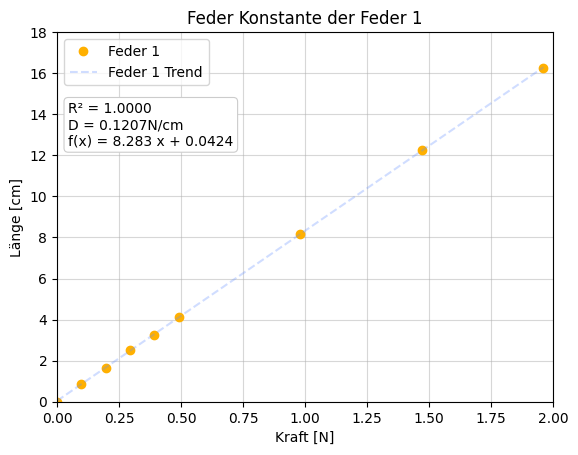
\includegraphics[scale=0.8]{graph/Spring-1}
    \caption{Graph von den gemessenen Werte von Feder 1 dargestellt und darstellung der Trendline}
    \label{fig:graph-spring-1}
\end{figure}
\begin{center}
    \begin{tabular}{ |l|r| } \hline
        Arithmetischer wert von \textmathbar{x}                             & 68.8426 cm            \\\hline
        Arithmetischer wert von s                                           & 0.0440 cm             \\\hline
        Arithmetischer wert von $\Delta$\textmathbar{x}                     & 0.0254 cm             \\\hline
        s des Mittelwertes von Mittelwert von s                             & 0.0147 cm             \\\hline
        Relativer Fehler von s Mittelert und Mittelwert von \textmathbar{x} & 0.0213 cm             \\\hline
        Streuung der Messwerte                                              & x = (x $\pm$ 0.04) cm \\\hline
        R\textsuperscript{2}                                                & 1.0000                \\\hline
        D                                                                   & 0.1207 N/cm           \\\hline
        f(x)                                                                & 8.283x + 0.0424       \\\hline
    \end{tabular}
\end{center}
\subsection{Feder 2}\label{subsec:statik-feder-2}
\begin{center}
    \begin{tabular}{ |l|l|l|l|l|l| }\hline\rowcolor{Gray!50}
        Index & \textmathbar{x} [cm]  & $\Delta$h [cm]        & s [cm]   & $\Delta$\textmathbar{x} [cm] & r [\%]  \\\toprule\hline
        0     & 74.11\textoverline{6} & 0.000                 & 0.028868 & 0.01\textoverline{6}         & 0.57735 \\\hline
        1     & 73.300                & 0.86\textoverline{6}  & 0.000000 & 0.000                        & 0.00000 \\\hline
        2     & 72.53\textoverline{3} & 1.58\textoverline{3}  & 0.057735 & 0.03\textoverline{3}         & 0.57735 \\\hline
        3     & 71.71\textoverline{6} & 2.400                 & 0.028868 & 0.01\textoverline{6}         & 0.57735 \\\hline
        4     & 71.91\textoverline{6} & 3.200                 & 0.028868 & 0.01\textoverline{6}         & 0.57735 \\\hline
        5     & 70.100                & 4.01\textoverline{6}  & 0.000000 & 0.000                        & 0.00000 \\\hline
        6     & 66.000                & 8.11\textoverline{6}  & 0.000000 & 0.000                        & 0.00000 \\\hline
        7     & 61.96\textoverline{6} & 12.150                & 0.057735 & 0.03\textoverline{3}         & 0.57735 \\\hline
        8     & 57.900                & 16.21\textoverline{6} & 0.100000 & 0.057735                     & 0.57735 \\\hline
    \end{tabular}
\end{center}
\begin{figure}[H]
    \centering
    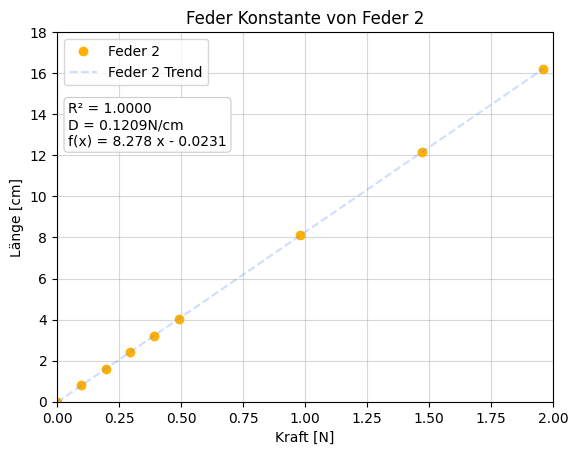
\includegraphics[scale=0.8]{graph/Spring-2}
    \caption{Graph von den gemessenen Werte von Feder 2 dargestellt und darstellung der Trendline}
    \label{fig:graph-spring-2}
\end{figure}
\begin{center}
    \begin{tabular}{ |l|r| } \hline
        Arithmetischer wert von \textmathbar{x}                             & 68.72\textoverline{7} cm \\\hline
        Arithmetischer wert von s                                           & 0.0336 cm                \\\hline
        Arithmetischer wert von $\Delta$\textmathbar{x}                     & 0.0194 cm                \\\hline
        s des Mittelwertes von Mittelwert von s                             & 0.0112 cm                \\\hline
        Relativer Fehler von s Mittelert und Mittelwert von \textmathbar{x} & 0.0163 cm                \\\hline
        Streuung der Messwerte                                              & x = (x $\pm$ 0.03) cm    \\\hline
        R\textsuperscript{2}                                                & 1.0000                   \\\hline
        D                                                                   & 0.1209 N/cm              \\\hline
        f(x)                                                                & 8.278x - 0.0231          \\\hline
    \end{tabular}
\end{center}
\subsection{Seriell}\label{subsec:statik-spring-series}
\begin{center}
    \begin{tabular}{ |l|l|l|l|l|l| }\hline\rowcolor{Gray!50}
        Index & \textmathbar{x} [cm]  & $\Delta$h [cm]        & s [cm]   & $\Delta$\textmathbar{x} [cm] & r [\%]  \\\toprule\hline
        0     & 54.63\textoverline{3} & 0.000                 & 0.057735 & 0.03\textoverline{3}         & 0.57735 \\\hline
        1     & 53.000                & 1.63\textoverline{3}  & 0.000000 & 0.000                        & 0.00000 \\\hline
        2     & 51.38\textoverline{3} & 3.250                 & 0.028868 & 0.01\textoverline{6}         & 0.57735 \\\hline
        3     & 49.83\textoverline{3} & 4.800                 & 0.057735 & 0.03\textoverline{3}         & 0.57735 \\\hline
        4     & 48.08\textoverline{3} & 6.550                 & 0.028868 & 0.01\textoverline{6}         & 0.57735 \\\hline
        5     & 46.43\textoverline{3} & 8.200                 & 0.057735 & 0.03\textoverline{3}         & 0.57735 \\\hline
        6     & 38.23\textoverline{3} & 16.400                & 0.057735 & 0.03\textoverline{3}         & 0.57735 \\\hline
        7     & 30.18\textoverline{3} & 24.450                & 0.076376 & 0.044096                     & 0.57735 \\\hline
        8     & 22.100                & 32.53\textoverline{3} & 0.100000 & 0.057735                     & 0.57735 \\\hline
    \end{tabular}
\end{center}
\begin{figure}[H]
    \centering
    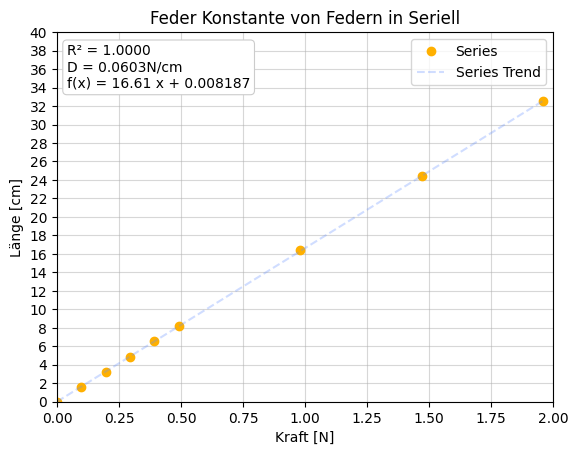
\includegraphics[scale=0.8]{graph/Spring-Series}
    \caption{Graph von den gemessenen Werte von Feder in Seriell dargestellt und darstellung der Trendline}
    \label{fig:graph-spring-series}
\end{figure}
\begin{center}
    \begin{tabular}{ |l|r| } \hline
        Arithmetischer wert von \textmathbar{x}                             & 43.7648 cm            \\\hline
        Arithmetischer wert von s                                           & 0.0517 cm             \\\hline
        Arithmetischer wert von $\Delta$\textmathbar{x}                     & 0.0298 cm             \\\hline
        s des Mittelwertes von Mittelwert von s                             & 0.0172 cm             \\\hline
        Relativer Fehler von s Mittelert und Mittelwert von \textmathbar{x} & 0.0394 cm             \\\hline
        Streuung der Messwerte                                              & x = (x $\pm$ 0.05) cm \\\hline
        R\textsuperscript{2}                                                & 1.0000                \\\hline
        D                                                                   & 0.0603 N/cm           \\\hline
        f(x)                                                                & 16.61x - 0.008187     \\\hline
    \end{tabular}
\end{center}
\subsection{Parallel}\label{subsec:statik-spring-parallel}
\begin{center}
    \begin{tabular}{ |l|l|l|l|l|l| }\hline\rowcolor{Gray!50}
        Index & \textmathbar{x} [cm]  & $\Delta$h [cm]       & s [cm]   & $\Delta$\textmathbar{x} [cm] & r [\%]  \\\toprule\hline
        0     & 73.83\textoverline{3} & 0.000                & 0.057735 & 0.03\textoverline{3}         & 0.57735 \\\hline
        1     & 73.500                & 0.33\textoverline{3} & 0.100000 & 0.057735                     & 0.57735 \\\hline
        2     & 73.03\textoverline{3} & 0.80                 & 0.057735 & 0.03\textoverline{3}         & 0.57735 \\\hline
        3     & 72.53\textoverline{3} & 1.300                & 0.057735 & 0.03\textoverline{3}         & 0.57735 \\\hline
        4     & 72.13\textoverline{3} & 1.700                & 0.057735 & 0.03\textoverline{3}         & 0.57735 \\\hline
        5     & 71.76\textoverline{6} & 2.06\textoverline{6} & 0.115470 & 0.06\textoverline{6}         & 0.57735 \\\hline
        6     & 69.73\textoverline{3} & 4.10                 & 0.057735 & 0.03\textoverline{3}         & 0.57735 \\\hline
        7     & 67.76\textoverline{6} & 6.06\textoverline{6} & 0.115470 & 0.06\textoverline{6}         & 0.57735 \\\hline
        8     & 65.800                & 8.03\textoverline{3} & 0.100000 & 0.057735                     & 0.57735 \\\hline
    \end{tabular}
\end{center}
\begin{figure}[H]
    \centering
    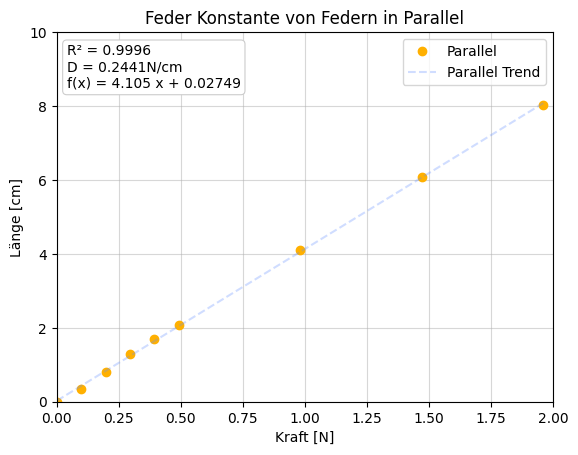
\includegraphics[scale=0.8]{graph/Spring-Parallel}
    \caption{Graph von den gemessenen Werte von Feder 1 dargestellt und darstellung der Trendline}
    \label{fig:graph-spring-parallel}
\end{figure}
\begin{center}
    \begin{tabular}{ |l|r| } \hline
        Arithmetischer wert von \textmathbar{x}                             & 71.12\textoverline{2} cm \\\hline
        Arithmetischer wert von s                                           & 0.0800 cm                \\\hline
        Arithmetischer wert von $\Delta$\textmathbar{x}                     & 0.0462 cm                \\\hline
        s des Mittelwertes von Mittelwert von s                             & 0.0267 cm                \\\hline
        Relativer Fehler von s Mittelert und Mittelwert von \textmathbar{x} & 0.0375 cm                \\\hline
        Streuung der Messwerte                                              & x = (x $\pm$ 0.08) cm    \\\hline
        R\textsuperscript{2}                                                & 0.9996                   \\\hline
        D                                                                   & 0.2441 N/cm              \\\hline
        f(x)                                                                & 4.105x + 0.02749         \\\hline
    \end{tabular}
\end{center}
\subsection{Feder Vergleiche}\label{subsec:statik-spring-comparisons}
\begin{figure}[H]
    \centering
    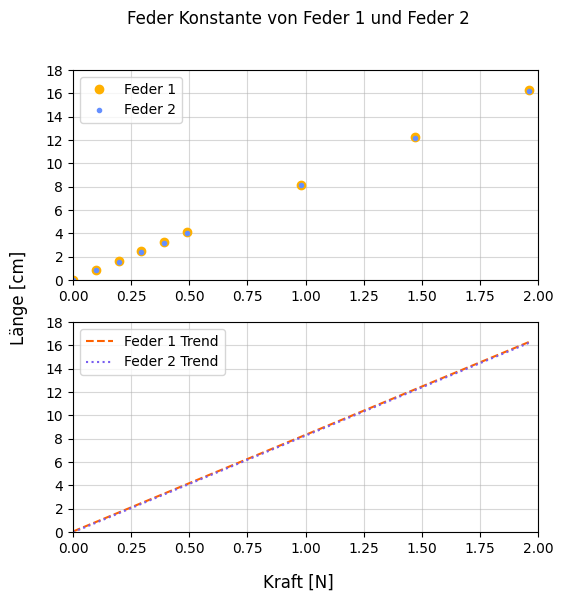
\includegraphics[scale=0.8]{graph/Spring-1-and-Spring-2}
    \caption{Die Darstellung der beiden gemessenen Federn übereinander gesetzt mit Datenpunkte und Trendlinie}
    \label{fig:graph-single-spring-comparisons}
\end{figure}
\begin{figure}[H]
    \centering
    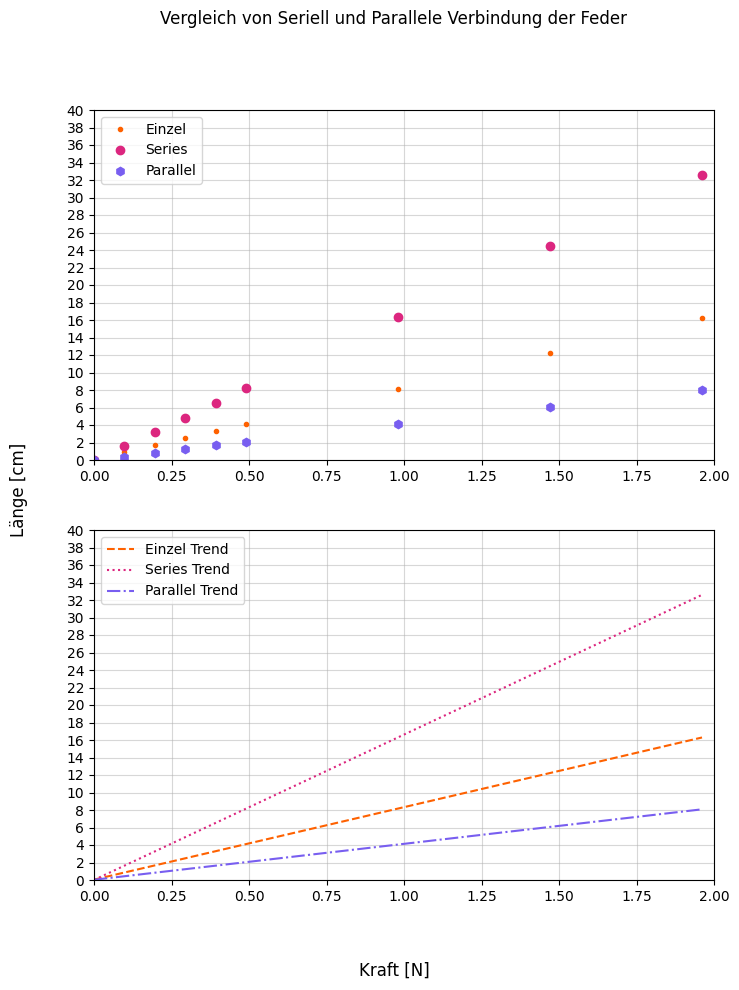
\includegraphics[scale=0.7]{graph/Spring-setup-comparison}
    \caption{Die Darstellung der Feder Positionen einzeln, in Seriell und in Parallel mit Datenpunkte und Trendlinien}
    \label{fig:graph-spring-setup-comparisons}
\end{figure}
\end{document}